\documentclass[11pt]{article}
% arXiv preprint (cs.DB; cross-list cs.IT). Compile: latexmk -pdf main.tex
\usepackage[T1]{fontenc}
\usepackage[utf8]{inputenc}
\usepackage[a4paper,margin=2.5cm]{geometry}
\usepackage{lmodern}
\usepackage{amsmath,amssymb,amsthm}
\usepackage{booktabs}
\usepackage{graphicx}
\graphicspath{{figures/}}
\usepackage{xcolor}
\usepackage{hyperref}
\usepackage[capitalise,noabbrev]{cleveref}
\usepackage{microtype}
\setlength{\emergencystretch}{2em}

\newtheorem{lemma}{Lemma}
\newtheorem{theorem}{Theorem}
\newtheorem{corollary}{Corollary}
\newtheorem{proposition}{Proposition}
\theoremstyle{definition}
\newtheorem{definition}{Definition}
\theoremstyle{remark}
\newtheorem{remark}{Remark}

\newcommand{\todo}[1]{\textcolor{red}{[TODO: #1]}}
\newcommand{\R}{\mathcal{R}}
\newcommand{\eps}{\varepsilon}
% Long identifiers may break after an underscore.
\newcommand{\code}[1]{\texttt{\let\_\codeus #1}}
\newcommand{\codeus}{\textunderscore\allowbreak}

\title{Alert-Preserving Lossy Compression of Monitoring Time Series}
\author{Bogdan Serykh\\
  Faculty of Computer Science, HSE University, Moscow, Russia\\
  \href{mailto:baserykh@edu.hse.ru}{\code{baserykh@edu.hse.ru}}\quad
  ORCID \href{https://orcid.org/0009-0007-0249-9959}{0009-0007-0249-9959}}
\date{November 2026\\[2pt]
  \small Preprint, \href{https://doi.org/10.5281/zenodo.24504704}{doi:10.5281/zenodo.24504704}}

\begin{document}
\maketitle

\begin{abstract}
Monitoring systems store large volumes of floating-point time series, and
most of these data are read only by alerting rules: threshold tests on
window aggregates with a hold duration. A lossy compressor with one error
bound for all samples either wastes space far from the thresholds or
changes alerts near them. We use the alert decisions as the correctness
criterion. For every rule, the reconstructed series must produce the same
sequence of alert states (\textsf{Inactive}, \textsf{Pending},
\textsf{Firing}) as the original, at any evaluation interval and phase.
For PromQL threshold rules over \code{last},
\code{avg/sum/min/max\_over\_time} and \code{rate} we derive a sound error
budget for each sample, computable in linear time. It is the smallest
value, over all windows that contain the sample, of the window's distance
to the threshold divided by a Lipschitz constant. Because the aggregates
are monotone, the budget splits into separate bounds for downward and
upward errors. For Prometheus' extrapolated \code{rate}, an
order-preserving quantizer leaves only the first and last sample of each
window constrained. Our codec combines predictive coding, a range coder and
a \emph{lazy} step choice that keeps the prediction whenever the budget
allows, which suits the asymmetric budget. After encoding, it decodes the
output, re-evaluates every rule and repairs any changed decision, so the
guarantee holds for the floating-point output. Parts of the
floating-point argument are machine-checked with Kani. On 13 real series
from the public Prometheus demo servers (7 and 30 days), the codec keeps
every alert decision (9\,055 firings) at 1.0--1.5 bits per value. This is
4--6.5 times less than a uniform bound tuned on the same data and less
than Compression Safeguards over SZ3 on 19 of 26 rule variants. In an
ablation, the one-sided budget and the lazy step choice together reduce
the size by a factor of 2.4--2.5.
\end{abstract}

\section{Introduction}
\label{sec:intro}

Monitoring systems such as Prometheus~\cite{prometheus} store large
volumes of floating-point time series (metrics). Few of the stored bytes
are ever read by a person. Most are read by alerting rules, which test a
window aggregate against a threshold, for example
\code{avg\_over\_time(x[5m]) > 0.8 for 10m} or
\code{rate(requests[5m]) < 20}.

Lossless time-series compressors of the Gorilla
family~\cite{pelkonen2015gorilla} spend 20--55 bits per value on typical
gauges, metrics such as load or memory use that move up and down
(\cref{def:kinds}). Error-bounded lossy compressors such as
SZ3~\cite{liang2023sz3} take a uniform pointwise bound $\eps$ and use it to
reduce the size. For alerting, one bound for all samples is a poor fit.
Far from a threshold almost any error is harmless. Near a threshold, an
error smaller than the measurement noise can create or suppress an alert.
A user who picks $\eps$ by hand therefore either wastes space or changes
which alerts fire without noticing.

We use the alert decisions themselves as the correctness criterion. A lossy
compressor is \emph{alert-preserving} for a rule set if every rule produces
the same alert state trajectory on the reconstruction as on the original,
that is, the same state (\code{Inactive}, \code{Pending} or \code{Firing})
at every evaluation. Any information the rules cannot observe can then be
discarded.

\paragraph{Contributions.}
\begin{itemize}
  \item A formal model of PromQL threshold alerts on a single series, with
    left-open windows, the \code{for}/\code{keep\_firing\_for} automaton
    and Prometheus' extrapolated \code{rate}. On this model we define
    decision preservation and \emph{phase robustness}, which requires
    preservation for every evaluation interval and phase without knowing
    how many samples a window holds (\cref{sec:model}).
  \item An error budget for each sample, derived from the rules
    (\cref{thm:budget}). An evaluation tolerates an error equal to its
    margin to the threshold divided by a Lipschitz constant of its
    aggregate, and a sample's budget is the smallest tolerance among the
    evaluations whose windows contain it. All aggregates except
    \code{rate} are monotone, so the budget splits into separate downward
    and upward bounds (\cref{cor:onesided}). For \code{rate} we show that
    counter resets make it discontinuous, and that under an
    order-preserving quantizer only the window ends need a budget
    (\cref{prop:rate}). The budget takes $O(n)$ time per rule.
  \item A codec that converts the asymmetric budget into a small stream
    (\cref{sec:codec}). It quantizes with closed-loop DPCM on power-of-two
    grids, chooses steps \emph{lazily} (it keeps the prediction when the
    budget allows), and codes the result with an adaptive binary range
    coder. A verify-and-repair loop compares the decoded output with a
    reference evaluator, so the guarantee holds in floating point. An
    optimistic variant starts from a multiple of the analytic budget and
    repairs only the evaluations that change, never going below the
    analytic budget.
  \item Bit-precise machine-checked proofs (Kani~\cite{vanhattum2022kani})
    of the floating-point budget for \code{last}, \code{min\_over\_time}
    and \code{max\_over\_time}, and of codec invariants
    (\cref{sec:verification}).
  \item An evaluation on synthetic series and on 13 real series from the
    public Prometheus demo servers with their upstream alert rules
    (\cref{sec:eval}). The 7- and 30-day snapshots are released with the
    code. We compare against uniform error bounds and against Compression
    Safeguards~\cite{tyree2026safeguards}, the closest existing system,
    and ablate every codec component.
\end{itemize}

\paragraph{Results.} On real data, no output of the rule-aware codec
changed any alert state, over 1\,864 firings in the 7-day snapshot and
7\,191 in the 30-day one. With thresholds that do fire, the codec needs
about 1--1.5 bits per value on real series. A uniform bound tuned by hand
on the same data needs 4--6.5 times more and still gives no guarantee on
other data. The codec is also smaller than Compression Safeguards over SZ3
on 19 of 26 real rule variants and on every synthetic one. In the
ablation, the one-sided budget and the lazy step choice together reduce
the size by a factor of 2.4--2.5.

The code and every table in this paper can be reproduced from
\url{https://github.com/ProgrammerPeasant/alert-preserving-compression}.
The real-series snapshots are archived at
\href{https://doi.org/10.5281/zenodo.24442344}{doi:10.5281/zenodo.24442344}~\cite{serykh2026snapshots}.

\section{Model and correctness criterion}
\label{sec:model}

\paragraph{Series.} A series is a finite sequence $X = ((s_i, x_i))_{i=1}^{n}$
with strictly increasing timestamps $s_i \in \mathbb{Z}$ (ms) and values
$x_i \in \mathbb{R}$. A value-only compressor keeps the timestamps and
returns $Y = ((s_i, y_i))$; the pointwise error is $e_i = y_i - x_i$.
Timestamps are compressed losslessly by existing delta-of-delta schemes and
are out of scope.

\paragraph{Rules.} A threshold rule is $R = (F, w, \bowtie, \theta, h, k)$:
an aggregate $F$, a range $w$, a comparison $\bowtie \in \{>, \ge, <, \le\}$,
a threshold $\theta$, a hold duration $h$ (\code{for}) and $k$
(\code{keep\_firing\_for}). It is the PromQL alert
\code{expr: F(x[w]) $\bowtie$ $\theta$} over one series. At evaluation time
$t$ the aggregate reads the samples with index in the support
$S_R(t) = \{ i : t - w < s_i \le t \}$ (range selectors are left-open in
Prometheus~3); for an instant selector (\code{last}) the support is the last
sample in $(t - \lambda, t]$ with lookback $\lambda = 5$\,min. The aggregate is
$f_R(X)(t) = F((x_i)_{i \in S_R(t)})$ and the condition is
$c_R(X)(t) = [S_R(t) \ne \emptyset \wedge f_R(X)(t) \bowtie \theta]$.

\paragraph{Decisions.} For an evaluation grid $T = (t_1 < t_2 < \dots)$ the
alert state trajectory $D_R(X) \in \{\mathsf{Inactive}, \mathsf{Pending},
\mathsf{Firing}\}^{|T|}$ is the run of the deterministic automaton
$M_{h,k}$ of Prometheus' \code{rules/alerting.go} on the condition sequence:
a true condition moves \textsf{Inactive} to \textsf{Pending}, and
\textsf{Pending} to \textsf{Firing} once it has held for $h$; a false
condition resets to \textsf{Inactive}, except that \textsf{Firing} persists
for $k$ after the condition was last true.

\begin{definition}[Decision preservation]
A compressor $C$ is \emph{decision-preserving} for a rule set $\R$ on $X$
over grid $T$ if $D_R(X) = D_R(C(X))$ for all $R \in \R$. It is
\emph{phase-robust} if this holds for every grid $T$.
\end{definition}

The criterion counts \textsf{Pending} periods as well as firings, so it is
stricter than ``the same alerts fire''. Relaxations (firing times within
$\delta$, firings only) admit larger budgets and are left for future work
(\cref{sec:conclusion}).

\begin{lemma}[Automaton]
\label{lem:automaton}
If $c_R(X)(t) = c_R(Y)(t)$ for all $t \in T$, then $D_R(X) = D_R(Y)$.
\end{lemma}
\begin{proof}
$M_{h,k}$ reads only $T$ and the condition sequence.
\end{proof}

\begin{lemma}[Phase robustness]
\label{lem:phase}
Let $F$ depend on $t$ only through $S_R(t)$ (true for \code{last} and
\code{avg/sum/min/max\_over\_time}) and let
$E = \{s_i\} \cup \{s_i + w\}$ ($s_i + \lambda$ for \code{last}). Then
$S_R(t)$, hence $c_R(X)(t)$, is constant between consecutive points of $E$
and empty before the first.
\end{lemma}
\begin{proof}
$i \in S_R(t) \iff s_i \le t < s_i + w$, so membership changes only at
$s_i$ or $s_i + w$.
\end{proof}

By \cref{lem:automaton,lem:phase}, preserving the conditions at the
\emph{protected instants} $P_R = E$ preserves the trajectories on every grid,
for any evaluation interval and phase, and $|E| \le 2n$. The encoder needs
the rule's range $w$, not the scrape interval or the number of samples per
window, so missed scrapes and irregular timestamps are covered. \code{rate}
depends on $t$ continuously through extrapolation and is protected on the
deployed grid $T$ only.

\section{Error budget}
\label{sec:budget}

\subsection{A sufficient condition}

For a protected evaluation $(R,t)$ with non-empty support let the margin be
$m_R(t) = |f_R(X)(t) - \theta|$ and let $L_R(t)$ be a Lipschitz constant of
$F$ on $\mathbb{R}^{|S_R(t)|}$ in the sup norm. \code{last},
\code{avg\_over\_time}, \code{min\_over\_time} and \code{max\_over\_time} have
$L = 1$; \code{sum\_over\_time} has $L = |S_R(t)|$. The tolerance of the
evaluation is $\tau_R(t) = m_R(t)/L_R(t)$ and the budget of sample $i$ is
the minimum over every evaluation that reads it:
\begin{equation}
  \eps_i = \min\{\tau_R(t) : R \in \R,\ t \in P_R,\ i \in S_R(t)\},
  \qquad \min\emptyset = +\infty .
  \label{eq:budget}
\end{equation}

The condition is $f_R(X)(t) \bowtie \theta$ or its negation, so on the
original data it is one of $f > \theta$, $f \ge \theta$, $f < \theta$,
$f \le \theta$. Two properties of this inequality matter below.

\begin{definition}[Tight, upper and lower evaluations]
\label{def:tight}
A protected evaluation $(R,t)$ is \emph{tight} if the inequality that holds
on $X$ is strict, i.e.\ $c_R(X)(t) = 1$ with ${\bowtie} \in \{>,<\}$, or
$c_R(X)(t) = 0$ with ${\bowtie} \in \{\ge,\le\}$. Then a reconstruction with
$f_R(Y)(t) = \theta$ already flips the condition, so the error must stay
strictly below the tolerance. It is \emph{upper} if $f_R(X)(t)$ lies on
the side of $\theta$ that only a decrease of the aggregate can leave
($c_R(X)(t) = 1$ with ${\bowtie} \in \{>,\ge\}$, or $c_R(X)(t) = 0$ with
${\bowtie} \in \{<,\le\}$), and \emph{lower} otherwise.
\end{definition}

We call the set of reconstructions
$\{Y : |y_i - x_i| \le \eps_i \text{ for all } i \in I\}$ the
\emph{box budget}: it bounds every error symmetrically.

\begin{theorem}[Box budget]
\label{thm:budget}
If $|y_i - x_i| \le \eps_i$ for all $i$, strictly on the supports of tight
evaluations, then $c_R(Y)(t) = c_R(X)(t)$ for all
$R \in \R$ and $t \in P_R$, and hence $D_R(Y) = D_R(X)$ on every grid (on $T$
for \code{rate}).
\end{theorem}
\begin{proof}
Supports depend on timestamps only. By the Lipschitz bound
$|f_R(Y)(t) - f_R(X)(t)| \le L_R(t)\max_{i\in S_R(t)}|e_i| \le m_R(t)$,
strictly when tight, so $f_R(Y)(t)$ stays on the same side of $\theta$.
\Cref{lem:phase,lem:automaton} finish the proof.
\end{proof}

The Lipschitz step is ordinary quantity-of-interest error
propagation~\cite{jiao2022qoi}. What is specific is the granularity: errors
live on samples and margins on evaluations, and one sample feeds every
evaluation whose window contains it, so the budget is a minimum over
overlapping windows. Two consequences follow. A streaming encoder needs a
lookahead of the longest window $\max_R w_R$, so the natural deployment point
is block compaction (Prometheus compacts 2-hour blocks) or a buffered proxy.
And a sample at margin zero must be exact. Since any smaller budget is also
sufficient, a pointwise cap $\min(\eps_i, \eps_{\max})$ adds a fidelity
guarantee for dashboards without weakening the alert guarantee.

\subsection{One-sided budget}

The box budget of \cref{thm:budget} is pessimistic: near a threshold a series
mostly lies on one side, and only errors towards $\theta$ can flip a
decision.

\begin{corollary}[One-sided budget]
\label{cor:onesided}
Let $\delta^-_i$ (the \emph{downward} budget) be the minimum of
$\tau_R(t)$ over the upper evaluations whose support contains $i$, and
$\delta^+_i$ (the \emph{upward} budget) the same minimum over the lower
ones, with $\min\emptyset = +\infty$ (\cref{def:tight}). If
$-\delta^-_i \le y_i - x_i \le \delta^+_i$ for all $i$ (strict where
tight), every protected condition is preserved.
\end{corollary}
\begin{proof}
All aggregates above are non-decreasing in each argument. For an upper
$(R,t)$ let $z_i = \min(y_i, x_i)$ on its support. Then
$|z_i - x_i| \le \delta^-_i \le \tau_R(t)$, so $z$ satisfies
\cref{thm:budget} at $(R,t)$, and $F(y) \ge F(z)$ keeps $f_R(Y)(t)$ on the
upper side. Lower evaluations are symmetric with $\max$.
\end{proof}

Since $\eps_i = \min(\delta^-_i, \delta^+_i)$, the box budget is contained in the
one-sided set, and the difference is large: a sample read only by upper
evaluations may move up without limit (\cref{fig:budget}). The coder exploits it only if it can
place reconstructions asymmetrically (\cref{sec:codec}); the ablation shows
that the one-sided budget alone, with round-to-nearest, gains little
(\cref{sec:ablation}).

\begin{figure}[t]
\centering
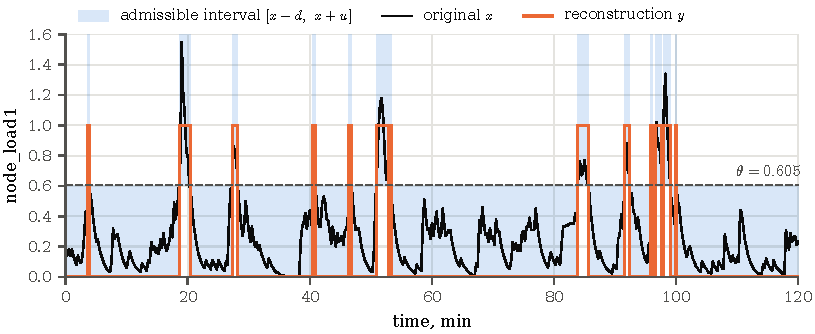
\includegraphics[width=\linewidth]{budget}
\caption{One-sided budget and the codec's reconstruction on two hours of
\code{node\_load1} (7-day snapshot, rule \code{last > }$\theta$ with $\theta$
at the 95th percentile). Below $\theta$ only the upward error is bounded,
above it only the downward one, so the admissible interval (shaded) is a
half-line and the reconstruction collapses to two levels; every alert
decision is unchanged.}
\label{fig:budget}
\end{figure}

\subsection{Counters and \code{rate}}
\label{sec:budget-rate}

We restate Prometheus' \code{rate} (\code{extrapolatedRate} in
\code{promql/functions.go}~\cite{promsrc}) for one evaluation $(R,t)$ with
$|S_R(t)| \ge 2$. Let $f$ and $l$ be the first and last indices of the
support $S_R(t)$. The rule reads:
\begin{itemize}
  \item the \emph{increase}
    $\Delta = x_l - x_f + \rho$, where
    $\rho = \sum_{i \in S_R(t),\, i > f,\, x_i < x_{i-1}} x_{i-1}$ adds back
    the value lost at every reset inside the window;
  \item the \emph{sampled interval} $\sigma = s_l - s_f$, the time covered
    by the samples;
  \item the \emph{extrapolation distances} $h_{\mathrm{s}}$ and
    $h_{\mathrm{e}}$ from the first and last sample to the window's start
    $t - w$ and end $t$, each replaced by half the mean sample spacing
    when it reaches $1.1$ times that spacing; they depend on timestamps
    only;
  \item the \emph{zero distance} $h_0 = \sigma x_f / \Delta$, the time
    before $s_f$ at which a counter growing at the window's average speed
    was zero (used only when $\Delta > 0$).
\end{itemize}
The increase is extrapolated to the window boundaries, but not past the
counter's zero point, and divided by the range in seconds:
\[
  \mathrm{rate} = \frac{\Delta}{w}\cdot
  \frac{\sigma + \min(h_{\mathrm{s}}, h_0) + h_{\mathrm{e}}}{\sigma}.
\]

\begin{proposition}
\label{prop:rate}
(a) The reset indicator $[x_i < x_{i-1}]$ is a comparison of two samples, so
an arbitrarily small error can create a reset and change $\Delta$ by a whole
counter value; no positive symmetric budget preserves \code{rate} in general.
(b) The closed-loop floor quantizer
$y_i = y_{i-1} + q\lfloor (x_i - y_{i-1})/q\rfloor$ (exact when the step
count would be negative) gives $x_i - q < y_i \le x_i$ and preserves
$x_i \ge x_{i-1} \Rightarrow y_i \ge y_{i-1}$; keeping the two samples
around each true reset exact preserves the reset set.
(c) On the reset-preserving set, $\mathrm{rate}$ is Lipschitz in
$(\Delta, x_f)$ away from $x_f = 0$, with constant
$\approx (2 + r)/w$ for a densely sampled window with $r$ resets.
(d) Under (b), $\Delta$ and $x_f$ read only the window's first and last
samples and the preserved reset values, so the budget of a \code{rate}
evaluation applies to the two ends of its window only.
\end{proposition}

The implementation does not use the constant in (c): it computes a sound
interval enclosure of the \code{rate} formula over the box
$y_i \in [x_i - \eps, x_i]$, including the zero-point branch, and finds the
largest safe $\eps$ by bisection. By (d), with a 30\,s evaluation grid on
15\,s scrapes about half of a counter's samples are no window's end and are
constrained only by monotonicity.

\subsection{Where no budget exists}

A positive budget exists at $x$ iff $x$ is interior to the set of inputs
with the same condition. Equality tests, \code{changes()}, \code{floor} and
\code{round} inside expressions, and label-selecting aggregations
(\code{topk}) violate this at their decision points and need exact samples
there; ratios and \code{histogram\_quantile} are locally Lipschitz and need
an interval enclosure like \code{rate}.

\subsection{Floating point and complexity}

The budget is computed in floating point. The code subtracts a rounding
slack from the margin: a floating-point sum of $n$ terms has error at most
$\gamma_{n-1}\sum_i|v_i|$ with $\gamma_n = nu/(1 - nu)$ and unit roundoff
$u = 2^{-53}$~\cite{higham2002accuracy}.
The code also uses the next representable value below the tolerance for strict
comparisons. Monotonicity holds bitwise for \code{last}, \code{min} and
\code{max}; Prometheus sums with Kahan compensation, which is not monotone,
so for \code{sum/avg} \cref{cor:onesided} goes through the error bound
instead, and an evaluation whose margin is within the rounding slack is
constrained in both directions.

Supports are monotone in $t$, so all supports follow by two pointers, window
aggregates by a two-stacks sliding queue, and the per-sample minimum in
\eqref{eq:budget} is a sliding minimum over instants (monotone deque). The
budget costs $O(n + |P_R|)$ per rule; \code{rate} adds a bisection of about
a dozen enclosure evaluations per instant.

\section{Codec}
\label{sec:codec}

The codec turns per-sample bounds $(\delta^-_i, \delta^+_i)$ into a
bit stream whose decoded values lie in the \emph{admissible interval}
\[
  A_i = [\,x_i - \delta^-_i,\ x_i + \delta^+_i\,].
\] A budget of zero (or NaN)
forces an exact sample; $+\infty$ leaves it unconstrained. The format does
not depend on the rules: the decoder sees only the stream.

\paragraph{Quantizer.} The lossy mode is closed-loop DPCM (differential
pulse-code modulation) on a grid of step $q = 2^e$. The prediction for
sample $i$ is the previous \emph{reconstruction}, $p_i = y_{i-1}$, not the
previous original value, so encoder and decoder predict identically and
errors do not accumulate. The reconstruction is $y_i = p_i + k_i q$ with
an integer \emph{step count} $k_i$, chosen from the admissible counts
\[
  K_i = \{\, k \in \mathbb{Z} : p_i + kq \in A_i \,\},
\]
which is non-empty whenever $q \le \delta^-_i + \delta^+_i$. The stream
stores either $k_i$ or its delta $k_i - k_{i-1}$.

\paragraph{Blocks.} The series is cut into blocks of 128 samples. For each
block the encoder picks the cheapest of (i) lossless Gorilla XOR
coding~\cite{pelkonen2015gorilla} and (ii) the quantizer above with one
exponent $e$ per block. The candidate exponents are, for each sample
of the block, the largest $e$ with $2^e \le \delta^-_i + \delta^+_i$ (so
that $K_i \ne \emptyset$; $2^e \le \delta^-_i$ for a counter), plus the three next finer grids, because the
coded size is not monotone in the step on discrete data; samples whose
interval the chosen grid may miss are escaped (below). For a counter the
quantizer is the floor quantizer of \cref{prop:rate}(b), which keeps the
reconstruction below the data and non-decreasing. A sample whose step count
would exceed $2^{50}$ in magnitude, or whose reconstruction misses $A_i$ in
floating point, is \emph{escaped}: stored as a raw 64-bit value.
The encoder checks every
reconstructed value against its bounds, so the bound holds for the actual
floating-point output, bit for bit as the decoder computes it.

\paragraph{Lazy steps.} The \emph{nearest} choice
$k_i = \mathrm{round}((x_i - p_i)/q)$ produces unbiased errors, which suits
a symmetric bound but wastes an asymmetric one. For every grid the encoder
also tries the \emph{lazy} choice: the $k \in K_i$ closest to zero (so
$y_i = p_i$ whenever the prediction is admissible) or closest to
$k_{i-1}$. With one-sided bounds the prediction stays
admissible for long runs, which the entropy coder turns into a few hundredths
of a bit per sample. Four strategies (nearest or lazy, coding counts or deltas)
are compared per block by exact coded cost.

\paragraph{Entropy coding.} Every block decision and residual is coded with
an LZMA-style adaptive binary range coder~\cite{martin1979range} with 15-bit
probabilities: each coded integer (step count or delta) is sent as a zero flag,
a sign and its bit length in unary, modelled in a context given by the
previous integer's magnitude, then its leading bit below the top one
(modelled) and the remaining bits (raw). Model rates
start fast and slow down with a count-based schedule, so short streams adapt
quickly. A fixed-width variant, storing each block's integers with the
block's maximal bit length, is kept for the ablation.

\paragraph{Chunks.} Prometheus cuts head chunks at 120 samples, and each must
decode on its own. The series can be coded as independent streams with 3--4
bytes of overhead each. The budget is still planned on the whole series,
since windows cross chunk boundaries. Counter chunks continue the previous
chunk's reconstruction as a floor, otherwise the output could drop at a
boundary and \code{rate} would see a spurious reset.

\paragraph{Verify and repair.} After encoding, the reconstruction is decoded
and every protected condition is re-evaluated with the reference semantics.
On any evaluation that flipped, the budget on its support is zeroed and the
series re-encoded. The loop terminates because an all-exact support reads the
original values. For \code{sum/avg} the verifier (sliding sum), the
reference evaluator (left-to-right) and Prometheus (Kahan) sum in different
orders, which differ by at most $2\gamma_{n-1}\sum|y_i|$ (\cref{sec:budget}); the verifier
therefore accepts an evaluation only if it lies farther than that from
$\theta$, or its support is bitwise exact. The analytic budget keeps twice
this margin and has needed no repair on any dataset; the loop makes the
guarantee end to end against the reference evaluator.

\paragraph{Optimistic budget.} The bounds of \cref{cor:onesided} hold for the
worst case of all errors at once; in window aggregates actual errors mostly
cancel. The encoder may start from $\kappa\delta^\pm_i$ with $\kappa > 1$:
on every flipped evaluation the budget on its support is halved, never below
the analytic budget, and zeroed once there. A support within the analytic
budget cannot flip (\cref{thm:budget}), so the analytic budget is both the
sound starting point at $\kappa = 1$ and the floor that bounds the number of
rounds. This is the codec-side counterpart of the correction approach of
Compression Safeguards~\cite{tyree2026safeguards}, restricted to the
supports that actually flipped.

\section{Machine-checked proofs}
\label{sec:verification}

\Cref{thm:budget} is a statement about real numbers; the code evaluates
margins, tolerances and aggregates in IEEE-754 double precision. We check the
floating-point implementation with Kani~\cite{vanhattum2022kani}, a bounded
model checker for Rust built on CBMC~\cite{kroening2014cbmc}, which encodes
floating-point operations bit-precisely. Harnesses quantify over all finite
inputs (and, where stated, NaN and infinities) of a fixed shape.

A monolithic harness for ``budget implies same condition'' over a window of
three samples does not finish in 6 hours for any aggregate: symbolic
execution is fast, but the final SAT query over the chain of floating-point
operations (aggregate, subtraction, \code{next\_down}, comparison) does not
close. We therefore prove \cref{thm:budget} for \code{last},
\code{min\_over\_time} and \code{max\_over\_time} compositionally, with an
abstract tolerance $\tau$ separating the expensive tolerance computation
from the window structure:
\begin{enumerate}
  \item[(A)] \emph{scalar tolerance}, one harness per comparison: if
    $\mathrm{fl}|y' - v| \le \tau(v)$, where $\tau$ is the implemented
    tolerance function, then $y'$ and $v$ are on the same side of $\theta$
    (31--39 min each);
  \item[(B)] \emph{window lemmas} on at most four variables: the extremum is
    attained by some sample; $\mathrm{fl}|y_j - x_k| \le
    \max(\mathrm{fl}|y_j - x_j|, \mathrm{fl}|y_k - x_k|)$ for the arg-extrema
    $j, k$ (99 and 116 min); rounded subtraction is monotone (65 min);
  \item[(C)] the implemented tolerance of a window equals
    $\tau(f(x))$ bitwise ($\le 1$ min), and the aggregates are monotone
    (\cref{cor:onesided}; 1--2 s).
\end{enumerate}
(A)--(C) compose to the floating-point version of \cref{thm:budget} for
these aggregates, for every window length. In addition, the decoder's
reconstruction is proved bit-identical to the encoder's for every block
parameter, including $-0.0$, together with the gauge and counter
invariants of the quantizer; zigzag and varint codes and the bit-level
specification of the bit I/O round-trip.

\paragraph{Not yet proved.} \code{sum/avg\_over\_time} need a rounded-sum
error lemma in place of (B); the range coder and the concrete bit writer
exhaust memory or time in symbolic execution (unbounded \code{Vec} growth,
a loop bound depending on a symbolic counter). These parts are covered by
property tests: round-trip tests of both formats with NaN, infinite and zero
budgets and counters, and $5 \times 2000$ randomised decision-preservation
cases cross-checked against a per-instant reference evaluator; a mutation
(budget $\times 3$) is caught. \todo{re-run \code{quantize\_matches\_decoder\_and\_budget}
after the one-sided change (harness updated, run time not recorded).}

\section{Evaluation}
\label{sec:eval}

\subsection{Setup}

\paragraph{Real data.} We use 13 series of raw 15\,s scrapes without gaps
from the public Prometheus demo servers~\cite{promdemo}. They include
node\_exporter gauges (load, available memory, free space on the root
filesystem, clock offset), counters and gauges of Prometheus itself, a
Caddy request counter and counters of a demo service. There are two
snapshots, of 7 days (40\,320 samples per series) and 30 days (172\,800
samples). The servers keep only 31 days of data, so we release the
snapshots with the code.

The demo server runs the upstream node-mixin and prometheus-mixin
alerts~\cite{nodemixin}. Nine of them read a single series once constant
denominators are folded into $\theta$. Counters without an upstream rule
get the rules \code{rate(x[5m]) > $\theta$ for 5m} and
\code{rate(x[5m]) < $\theta$ for 10m}. On a healthy host the deployed
thresholds (\code{prod}) never fire. We therefore also run every series
with two recalibrated thresholds, computed from the rule's own aggregate:
the 95th percentile (\code{q95}, an alert that fires often) and the median
(\code{q50}, where the aggregate crosses $\theta$ all the time). Each such
threshold is placed midway between two distinct values, so that discrete
metrics never sit exactly on $\theta$. This gives 26 rule variants per
snapshot, with 1\,864 firings over 7 days and 7\,191 over 30 days.

\paragraph{Synthetic data.} Five seeded generators produce 7 days of
data at 15\,s: CPU utilisation, request latency, memory, a request
counter, and the same counter with 8\,\% missed scrapes, outages of
1--6\,min and traffic that stays close to the threshold. Each dataset has
two rules that fire a few times per day.

\paragraph{Evaluation.} Rules are evaluated every 30\,s, 7\,s after the
scrapes. We compare full alert state trajectories, computed by the
reference evaluator in the repository, which implements Prometheus~3
semantics. Sizes are in bits per value of the value stream, without
timestamps; an uncompressed value takes 64 bits.

\paragraph{Baselines.} Our own configurations all use the same codec and
range coder and differ only in the error budget. \emph{Lossless} is the
codec with a zero budget, which yields Gorilla XOR blocks.
\emph{Uniform-safe} is the largest uniform bound that satisfies
\cref{thm:budget}. \emph{Uniform-tuned} is found by sweeping uniform
bounds over powers of four of the value range: it is the largest bound
such that neither it nor any smaller bound in the sweep changes a decision
\emph{on these data}. A user tuning a bound by hand could do no better,
and the bound guarantees nothing on other data. \emph{SZ3+SG} is
SZ3~\cite{liang2023sz3} wrapped in Compression
Safeguards~\cite{tyree2026safeguards} (1.0.0rc3). It has one stencil
quantity of interest for every window length the rule can read at any
phase, with the comparison itself as the quantity and bound zero. We sweep
13 SZ3 bounds and report the smallest output among those that change no
decision. \emph{Rule-aware} is the analytic budget (\cref{cor:onesided}),
and \emph{$\kappa$} is the optimistic budget with $\kappa = 1024$.

\subsection{Real series}
\label{sec:eval-real}

\begin{table}[t]
\centering
\caption{Mean bits per value over the 13 real series. Zero changed decisions
in every rule-aware cell. ``/120'': Prometheus-sized independent chunks.}
\label{tab:real}
\begin{tabular}{llrrrrrrr}
\toprule
 & rules & lossless & unif.-safe & unif.-tuned & rule-aware & $\kappa$ & rule-aware/120 & $\kappa$/120 \\
\midrule
7\,d  & prod & 27.71 & 0.08 & 0.09 & 0.07 & 0.07 & 0.45 & 0.42 \\
      & q95  & 25.52 & 6.91 & 7.29 & 1.13 & 1.00 & 1.77 & 1.59 \\
      & q50  & 25.52 & 7.69 & 6.01 & 1.49 & 1.38 & 2.16 & 2.00 \\
\midrule
30\,d & prod & 27.77 & 0.08 & 0.08 & 0.06 & 0.06 & 0.44 & 0.41 \\
      & q95  & 25.59 & 7.99 & 5.72 & 0.96 & 0.86 & 1.58 & 1.43 \\
      & q50  & 25.59 & 7.47 & 5.91 & 1.15 & 1.08 & 1.80 & 1.68 \\
\bottomrule
\end{tabular}
\end{table}

\Cref{tab:real} summarises the real data. With the deployed thresholds
nothing fires, and every codec, including the uniform ones, needs less
than 0.1 bits per value, because a threshold that the data never approach
constrains nothing. This is the usual situation in production, but it
does not distinguish the methods. With the recalibrated thresholds, the
rule-aware codec is smaller than the tuned uniform bound by a factor of
6.5 (q95) and 4.0 (q50) on 7 days, and 6.0 and 5.1 on 30 days. Unlike the
tuned bound, it also guarantees the decisions. Per series, its size ranges
from 0.01 bits per value for free filesystem space, which rarely changes,
to 3--4.5 for dense counters under \code{rate} with the median threshold.
In Prometheus-sized chunks of 120 samples, the size grows by 0.6--0.7 bits
per value, mostly because of the fixed overhead per chunk and because the
models start each chunk untrained.

\subsection{Comparison with Compression Safeguards}
\label{sec:eval-sg}

\begin{figure}[t]
\centering
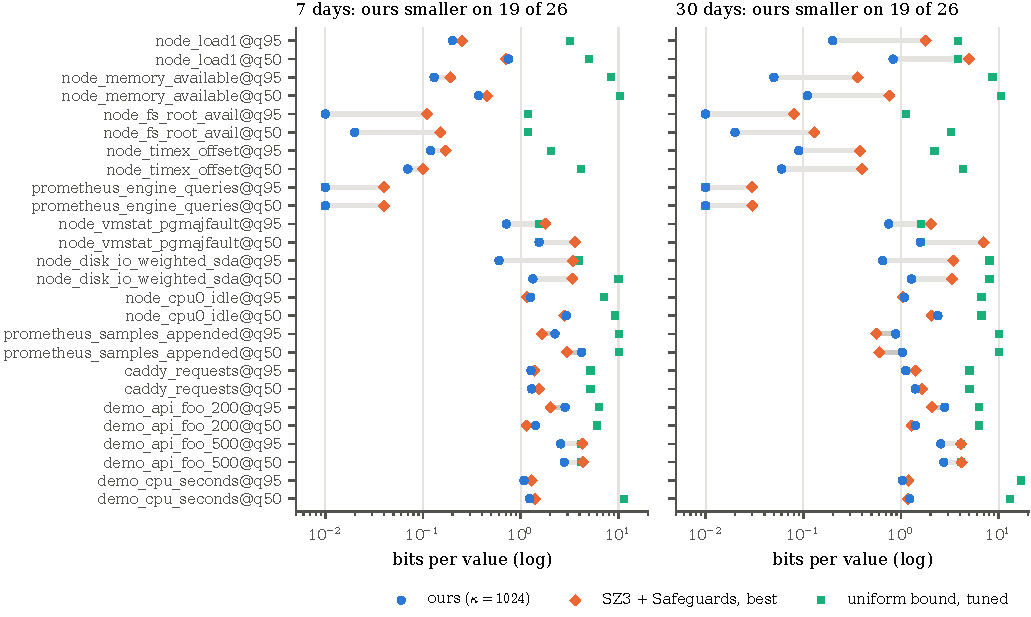
\includegraphics[width=\linewidth]{sg}
\caption{Bits per value on the real series: our optimistic codec
($\kappa = 1024$), the smallest SZ3+SG output with no changed decision over
its bound sweep, and our codec with the largest uniform bound that keeps
every decision on these data (tuned, no guarantee). A grey bar joins ours
to SZ3+SG.}
\label{fig:sg}
\end{figure}

The optimistic codec is smaller than SZ3+SG on 19 of 26 variants in both
snapshots (\cref{fig:sg}). The geometric mean of the size ratio
$\kappa$/SG is 0.60 on 7 days and 0.42 on 30 days. SG stays smaller on
dense counters under \code{rate}
(\code{prometheus\_samples\_appended}, \code{node\_cpu0\_idle} and
\code{demo\_api\_foo\_200}). On these series our quantizer uses one step
for a whole 128-sample block, while SG corrects individual samples.

SG's translation of \code{rate} cannot express Prometheus' extrapolation.
It changed decisions at some sweep points on 4 of the 8 real counters
across the two snapshots, and at 11 of 13 sweep points on the synthetic
counter with missed scrapes. On that counter, the smallest SG output that
keeps every decision takes 8.45 bits per value, 2.9 times more than our
analytic codec (2.91) and 3.1 times more than our optimistic codec (2.74).
A user cannot tell in advance which SG bound is safe. SG needs up to 60\,s per sweep
point on a 30-day counter, while our whole verified codec runs at
11--16\,MB/s (\cref{sec:throughput}).

\subsection{Synthetic series}

\begin{table}[t]
\centering
\caption{Synthetic series, 7 days, bits per value (one stream per series).
SZ3+SG: smallest output with zero changed decisions over its sweep.}
\label{tab:synth}
\begin{tabular}{lrrrrrr}
\toprule
dataset & lossless & unif.-safe & unif.-tuned & SZ3+SG & rule-aware & $\kappa$ \\
\midrule
cpu            & 53.96 & 11.57 & 2.55 & 0.16 & 0.07 & 0.05 \\
latency        & 55.24 &  7.22 & 2.81 & 0.20 & 0.08 & 0.07 \\
memory         & 49.91 & 12.96 & 6.92 & 0.57 & 0.21 & 0.14 \\
requests       & 19.68 &  2.02 & 0.78 & 0.69 & 0.35 & 0.35 \\
requests-gappy & 21.76 & 11.46 & 9.46 & 8.45 & 2.91 & 2.74 \\
\bottomrule
\end{tabular}
\end{table}

On the synthetic gauges (\cref{tab:synth}) the rule-aware codec is
33--36 times smaller than the tuned uniform bound, and on the counters
2.2 and 3.2 times smaller. The analytic codec is smaller than SZ3+SG on
all five datasets. With the box budget of \cref{thm:budget} it was larger
than SZ3+SG on the three gauges, and this result led us to
\cref{cor:onesided}. The size grows with the share of samples near a
threshold: on \code{cpu}, it goes from 0.01 to 0.66 bits per value as that
share goes from 0.1\,\% to 10\,\% (\cref{fig:h2}).

\begin{figure}[t]
\centering
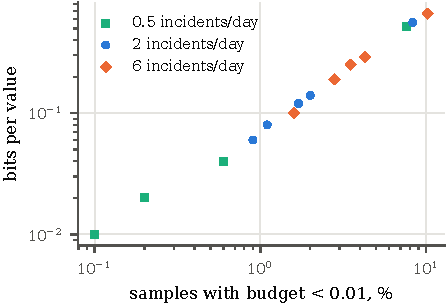
\includegraphics[width=0.5\linewidth]{h2}
\caption{Size of the rule-aware codec on synthetic \code{cpu} (7 days,
one rule) against the share of samples whose budget is below 0.01, for
$\theta \in \{0.55, \dots, 0.95\}$ and three incident rates.}
\label{fig:h2}
\end{figure}

\paragraph{Fidelity.} Without a cap, the reconstruction is useful only
for the rules, since a sample that is free in one direction drifts until
a bound stops it. With a pointwise cap $\eps_{\max}$, the rule-aware
codec is within 2\,\% of the size of a uniform bound $\eps_{\max}$ and
keeps every decision. A uniform bound of $10^{-3}$ of the range changes
17, 929 and 10\,655 alert states on \code{memory}, \code{requests} and
\code{requests-gappy}. Even the tuned uniform bound changes decisions on
two datasets when it is applied to 120-sample chunks instead of the
whole-series encoding it was tuned on. A bound tuned on one encoding of
the data does not carry over to another encoding of the same data.

\subsection{Ablation}
\label{sec:ablation}

\begin{table}[t]
\centering
\caption{Ablation: geometric mean of the size ratio to the full analytic
codec (row 3) over the synthetic series and the q95/q50 real variants
(7-day snapshot; the 30-day snapshot, in the repository, shows the same
ordering). Every cell keeps every
decision.}
\label{tab:ablation}
\begin{tabular}{lrrr}
\toprule
configuration & synthetic & real q95 & real q50 \\
\midrule
box budget, nearest steps (\cref{thm:budget}) & 2.44 & 2.53 & 2.47 \\
\quad + one-sided budget (\cref{cor:onesided}) & 2.27 & 2.06 & 1.91 \\
\quad + lazy steps (full analytic codec) & 1.00 & 1.00 & 1.00 \\
\quad + optimistic budget, $\kappa = 1024$ & 0.80 & 0.92 & 0.95 \\
full analytic + budget-scale search & 1.00 & 1.00 & 1.00 \\
full analytic $-$ one-sided budget & 1.37 & 1.21 & 1.20 \\
full analytic $-$ lazy steps & 2.27 & 2.06 & 1.91 \\
$\kappa = 1024$ $-$ one-sided budget & 0.93 & 1.05 & 1.08 \\
full analytic, fixed-width codes & 8.01 & 7.37 & 5.92 \\
\bottomrule
\end{tabular}
\end{table}

\Cref{tab:ablation} adds one component at a time. With the same stream
format, the one-sided budget and the lazy step choice reduce the size by
a factor of 2.4--2.5 when used together. Either one alone gains much
less. With round-to-nearest, the grid is chosen from the width of the
admissible interval and rounding uses that width symmetrically, so
one-sided bounds alone gain little and sometimes make the output larger.
On counters, all of the gain comes from lazy steps, which keep the
prediction on samples that are not the end of any window
(\cref{prop:rate}(d)). We had also encoded scaled copies of the budget
($\times\frac12, \frac14, \frac18$), because the coded size is not
monotone in the budget. Once the encoder tries the three next finer grids
per block, this search is redundant: it gives a smaller output on none of
the 31 datasets, so the codec no longer does it. The optimistic budget
saves a further 4--20\,\%, but on real data it does not replace the
one-sided budget. Entropy coding avoids the minimum of one bit per value
of fixed-width codes and makes the output 5.9--8.6 times smaller over
both snapshots.

\subsection{Throughput}
\label{sec:throughput}

We measure throughput on one core, in MB/s of raw float64 input, on
synthetic \code{cpu} and \code{requests} with 40\,320 samples. The $O(n)$
budget computation runs at 42--67\,MB/s. The encoder runs at 22\,MB/s,
since every block tries four grids with four step strategies each, and
the decoder at 2.5--2.9\,GB/s. The whole verified compressor runs at
11--16\,MB/s, or 3--4\,MB/s with the budget-scale search, which no longer
changes the size (\cref{sec:ablation}). A 2-hour Prometheus block holds
480 samples per series at 15\,s, so one core compresses about 2\,900
series-blocks per second.

\section{Related work}
\label{sec:related}

\paragraph{Correction-based safeguards.} Compression
Safeguards~\cite{tyree2026safeguards} wrap any compressor with declarative
requirements, such as pointwise bounds, sign preservation relative to an
offset, or bounds on quantities of interest over stencils. After
compression they compute corrections that enforce the requirements. A
window-average threshold test on a regular grid can be written as a stencil
quantity of interest: the quantity is the comparison itself and its bound
is zero. We run Safeguards this way as a baseline (\cref{sec:eval-sg}).

The two approaches differ in what has to be translated into the
requirement language and in how the requirement is enforced. Our
criterion needs no translation of hold durations (\cref{lem:automaton}),
but a stencil does need one for phase robustness. A stencil fixes the
window length in samples, so missed scrapes and an unknown evaluation
phase require one stencil for every window length that occurs, plus
truncated windows at the edges. Prometheus' \code{rate} extrapolation and
counter resets (\cref{prop:rate}) have no stencil form at all. The
translation we use for the baseline, the reset-corrected increase over the
sampled interval, changes decisions on counters with gaps. Safeguards
correct every point that violates a requirement. Our analytic budget is
sound from the start and needs no correction, and our optimistic variant
corrects only the supports whose evaluations changed, never going below
the analytic budget.

\paragraph{Quantity-of-interest preservation.} Jiao et
al.~\cite{jiao2022qoi} derive pointwise error bounds from bounds on derived
quantities by error propagation, and our Lipschitz step is one instance of
their method. We bound a decision instead of the error of a quantity, so
our budget depends on the distance to a threshold. We also handle the
structure in time: overlapping windows, evaluation phase and the alert
automaton.

\paragraph{Feature- and topology-preserving compression.} TopoSZ and its
successors~\cite{yan2024toposz} preserve critical points and contour trees
of scientific fields, and adaptive schemes tighten the bounds near
detected features~\cite{adaptivefeature2024}. Preserving the level set at
$\theta$ means preserving the sign of $x - \theta$, which is our setting
restricted to \code{last}. Window aggregates and alert states have no
counterpart in that work.

\paragraph{Time-series compression.} Gorilla~\cite{pelkonen2015gorilla} and
ALP~\cite{afroozeh2024alp} are lossless. SZ3~\cite{liang2023sz3} and recent
error-bounded time-series compressors~\cite{shrink2025} guarantee a uniform
pointwise bound. CAMEO~\cite{cameo2025} bounds the deviation of
autocorrelation functions, and Muñiz-Cuza et
al.~\cite{munizcuza2024forecasting} measure how error-bounded compression
affects forecasting. Plato~\cite{lin2020plato} gives deterministic error
bounds on aggregate queries over compressed series, which bound the
numeric result of a query. None of these systems bounds which side of a
threshold a result falls on, so none of them preserves discrete decisions.

\paragraph{Downstream guarantees and industrial practice.} Outside time
series, the closest guarantee we know is cluster preservation for particle
data~\cite{ren2026clusters}. Friends-of-friends cluster membership depends
on threshold tests on distances, and a correction applied after
compression, within the pointwise bound, restores it, much as our repair
loop restores changed evaluations. Industrial cost controls choose which
series to keep instead of bounding their values. Grafana's Adaptive
Metrics recommends aggregating away labels that no dashboard, rule or
recent query uses, and makes no recommendation for a metric that a
recording or alerting rule reads~\cite{grafana2026adaptive}. Our method
targets those metrics. We searched the literature (Crossref, arXiv,
EDBT/VLDB proceedings, 2015--2026) and vendor documentation and found no
compressor that guarantees alert decisions.

\section{Limitations and future work}
\label{sec:conclusion}

\paragraph{Scope of the rules.} We handle one series per rule. Aggregations
across series (\code{sum by}) couple the budgets of a group, which the
encoder must then see together; ratios need an interval enclosure; equality
tests and \code{topk} admit no positive budget at their decision points.

\paragraph{Known rules.} The budget is computed for a fixed rule set. A rule
added later sees a reconstruction that was optimised for other rules, with
only the optional pointwise cap as a guarantee. Re-compressing from the
original is possible while it is retained (e.g.\ before compaction).

\paragraph{Lookahead.} The budget of a sample depends on evaluations up to
one window after it, so the encoder must buffer the longest window; it fits
compaction or a buffered proxy, not a zero-latency write path.

\paragraph{Data.} Our real data come from two public demo servers: 13 series,
with thresholds recalibrated to quantiles because the deployed ones never
fire. Production traces with more rules, more incidents and gaps are needed.

\paragraph{Relaxations.} Counting \textsf{Pending} periods makes the
criterion strict. Preserving firings only, or firing times up to $\delta$,
admits budgets above the margin on short condition flips (\code{for}
filters them), at the cost of reasoning on the automaton rather than per
evaluation. The min-composition in \eqref{eq:budget} is feasible but not
optimal: for linear aggregates the optimal split of a margin between samples
is a knapsack-like problem.

\section{Conclusion}

Taking alert decisions as the correctness criterion turns lossy
compression of monitoring data into a problem with a sound, computable,
per-sample budget. Monotonicity of the aggregates makes the budget
one-sided, and a coder that can keep its prediction whenever it is still on
the admissible side converts that into a 2.4--2.5$\times$ smaller
output than the symmetric Lipschitz box. On
real Prometheus series the result is a few tenths to a few bits per value
with every alert decision unchanged.


\bibliographystyle{plainurl}
\bibliography{refs}

\end{document}
